\chapter{Infrastructure Setup and Installation} 
% Main appendix title

\label{AppendixA} 
% Change X to a consecutive letter; for referencing this appendix elsewhere, use \ref{AppendixX}

\lhead{Appendix A. \emph{Infrastructure Setup and Installation}} 
% Change X to a consecutive letter; this is for the header on each page - perhaps a shortened title

% Write your Appendix content below here.
% =========================================

\section{Linux command for Go compiler installation}
\lstset{basicstyle=\ttfamily\tiny} 
\begin{lstlisting}[breaklines, frame=single, numbers=left, caption={Linux command for Golang compiler installation}, label=commandline-02]       

===========================================================
(1) DOWNLOAD GOLANG go1.8.3.linux-amd64.tar.gz
AT URL https://golang.org/dl/ USING wget IN TERMINAL
=========================================================== 

yinghua@yinghua-NL8C:~/Downloads/temp$ wget -c https://storage.googleapis.com/golang/go1.8.3.linux-amd64.tar.gz
... 
go1.8.3.linux-amd64 100%[===================>]  85.86M  5.93MB/s    in 14s     
yinghua@yinghua-NL8C:~/Downloads/temp$

==========================================================
(2) EXTRACT DOWNLOADED SOURCE
==========================================================
yinghua@yinghua-NL8C:~/Downloads/temp$ tar -xzvf go1.8.3.linux-amd64.tar.gz 
.... 
yinghua@yinghua-NL8C:~/Downloads/temp$

==========================================================
(3) MOVE AND RENAME GOLANG DIRECTORY
==========================================================
yinghua@yinghua-NL8C:~/Downloads/temp$ mkdir -p ~/Desktop/apps/golang1.8.3
yinghua@yinghua-NL8C:~/Downloads/temp$ mv go ~/apps/golang1.8.3
yinghua@yinghua-NL8C:~/Downloads/temp$

==========================================================
(4) CHECK GOLANG DIRECTORY
==========================================================
yinghua@yinghua-NL8C:~/Downloads/temp$ cd ~/Desktop/apps/ 
yinghua@yinghua-NL8C:~/Desktop/apps$ ls -l
total 24
drwxr-xr-x  8 yinghua yinghua 4096 Sep 11 03:03 eclipse-oxygen
drwxrwxr-x  4 yinghua yinghua 4096 Sep  7 23:19 eclipse-workspace
drwxr-xr-x 11 yinghua yinghua 4096 May 25 02:16 golang1.8.3

==========================================================
(5) GO INTO GOLANG INSTALLED DIRECTORY
==========================================================
yinghua@yinghua-NL8C:~/Desktop/apps$ cd golang1.8.3/
yinghua@yinghua-NL8C:~/Desktop/apps/golang1.8.3$ ls -l
total 160
drwxr-xr-x  2 yinghua yinghua  4096 May 25 02:15 api
-rw-r--r--  1 yinghua yinghua 33243 May 25 02:15 AUTHORS
drwxr-xr-x  2 yinghua yinghua  4096 May 25 02:16 bin
drwxr-xr-x  4 yinghua yinghua  4096 May 25 02:16 blog
-rw-r--r--  1 yinghua yinghua  1366 May 25 02:15 CONTRIBUTING.md
....
yinghua@yinghua-NL8C:~/Desktop/apps/golang1.8.3$

=========================================================
(5.1) CHECK GOLANG EXECUTABLES
=========================================================
yinghua@yinghua-NL8C:~/Desktop/apps/golang1.8.3$ ls -al bin
total 28120
drwxr-xr-x  2 yinghua yinghua     4096 May 25 02:16 .
drwxr-xr-x 11 yinghua yinghua     4096 May 25 02:16 ..
-rwxr-xr-x  1 yinghua yinghua 10073055 May 25 02:16 go
-rwxr-xr-x  1 yinghua yinghua 15226597 May 25 02:16 godoc
-rwxr-xr-x  1 yinghua yinghua  3481554 May 25 02:16 gofmt
yinghua@yinghua-NL8C:~/Desktop/apps/golang1.8.3$


=========================================================
(5.2) CHECK GOLANG LIBRARIES
=========================================================
yinghua@yinghua-NL8C:~/Desktop/apps/golang1.8.3$ ls -al lib
total 12
drwxr-xr-x  3 yinghua yinghua 4096 May 25 02:15 .
drwxr-xr-x 11 yinghua yinghua 4096 May 25 02:16 ..
drwxr-xr-x  2 yinghua yinghua 4096 May 25 02:15 time
yinghua@yinghua-NL8C:~/Desktop/apps/golang1.8.3$

=========================================================
(5.3) CHECK GOLANG PACKAGES
=========================================================
yinghua@yinghua-NL8C:~/Desktop/apps/golang1.8.3$ ls -al pkg
total 28
drwxr-xr-x  7 yinghua yinghua 4096 May 25 02:16 .
drwxr-xr-x 11 yinghua yinghua 4096 May 25 02:16 ..
drwxr-xr-x  2 yinghua yinghua 4096 May 25 02:15 include
drwxr-xr-x 30 yinghua yinghua 4096 May 25 02:16 linux_amd64
yinghua@yinghua-NL8C:~/Desktop/apps/golang1.8.3$
....

==========================================================
(6) SET PATH TO GOLANG BINARY EXECUTABLES AND EXPORT PATH
==========================================================
yinghua@yinghua-NL8C:~/Desktop/apps/golang1.8.3$ cd bin
yinghua@yinghua-NL8C:~/Desktop/apps/golang1.8.3/bin$ pwd
/home/yinghua/Desktop/apps/golang1.8.3/bin
yinghua@yinghua-NL8C:~/Desktop/apps/golang1.8.3/bin$ export PATH=/home/yinghua/Desktop/apps/golang1.8.3/bin:$PATH
yinghua@yinghua-NL8C:~/Desktop/apps/golang1.8.3/bin$

==========================================================
(6.1) CHECK ADDED GOLANG PATH
==========================================================
yinghua@yinghua-NL8C:~/Desktop/apps/golang1.8.3/bin$ echo $PATH
/home/yinghua/Desktop/apps/golang1.8.3/bin: <=== PATH ADDED
/home/yinghua/.cargo/bin:
/home/yinghua/bin:
/home/yinghua/.local/bin:
/usr/local/sbin:
....
yinghua@yinghua-NL8C:~/Desktop/apps/golang1.8.3/bin$


==========================================================
(6.2) SET GOROOT AND GOPATH
==========================================================
yinghua@yinghua-NL8C:~/Desktop/apps/golang1.8.3/bin$ mkdir ~/Desktop/apps/gopath
yinghua@yinghua-NL8C:~/Desktop/apps/golang1.8.3/bin$ ls -al ~/Desktop/apps
total 24
drwxr-xr-x  8 yinghua yinghua 4096 Sep 11 03:03 eclipse-oxygen
drwxrwxr-x  4 yinghua yinghua 4096 Sep  7 23:19 eclipse-workspace
drwxr-xr-x 11 yinghua yinghua 4096 May 25 02:16 golang1.8.3
drwxrwxr-x  5 yinghua yinghua 4096 Sep  7 23:05 gopath

yinghua@yinghua-NL8C:~/Desktop/apps/golang1.8.3/bin$ export GOROOT=/home/yinghua/Desktop/apps/golang1.8.3
yinghua@yinghua-NL8C:~/Desktop/apps/golang1.8.3/bin$ export GOROOT=/home/yinghua/Desktop/apps/gopath
yinghua@yinghua-NL8C:~/Desktop/apps/golang1.8.3/bin$ export PATH=$GOPATH/bin:$PATH

==========================================================
(6.3) CHECK GOROOT AND GOPATH
==========================================================
yinghua@yinghua-NL8C:~/Desktop/apps/golang1.8.3/bin$ echo $GOROOT
/home/yinghua/Desktop/apps/golang1.8.3
yinghua@yinghua-NL8C:~/Desktop/apps/golang1.8.3/bin$ echo $GOPATH
/home/yinghua/Desktop/apps/gopath
yinghua@yinghua-NL8C:~/Desktop/apps/golang1.8.3/bin$ 

==========================================================
(6.4) APPLY SYSTEM UPDATES
==========================================================
yinghua@yinghua-NL8C:~/Desktop/apps/golang1.8.3/bin$ sudo updatedb
[sudo] password for yinghua: 
yinghua@yinghua-NL8C:~/Desktop/apps/golang1.8.3/bin$ sudo ldconfig
yinghua@yinghua-NL8C:~/Desktop/apps/golang1.8.3/bin$ sudo depmod
yinghua@yinghua-NL8C:~/Desktop/apps/golang1.8.3/bin$

===========================================================
(7) APPEND PATH TO USER PROFILE .bashrc FILE
===========================================================
yinghua@yinghua-NL8C:~/Desktop/apps/golang1.8.3/bin$ nano ~/.bashrc

# ======= ADDED BY CYH INTO ~/.bashrc ============
# added by CYH for Golang1.8.3 Compiler
export GOROOT=/home/yinghua/Desktop/apps/golang1.8.3
export GOPATH=/home/yinghua/Desktop/apps/gopath
export PATH=$GOROOT/bin:$GOPATH/bin:$PATH

===========================================================
(8) CHECK GO EXECUTABLE AND GO VERSION
===========================================================
yinghua@yinghua-NL8C:~/Desktop/apps/golang1.8.3/bin$ which go
/home/yinghua/Desktop/apps/golang1.8.3/bin/go
yinghua@yinghua-NL8C:~/Desktop/apps/golang1.8.3/bin$ go version
go version go1.8.3 linux/amd64
yinghua@yinghua-NL8C:~/Desktop/apps/golang1.8.3/bin$ 

==========================================================
(9) TEST GO EXECUTABLE
==========================================================
yinghua@yinghua-NL8C:~/Desktop/apps/golang1.8.3/bin$ go help
Go is a tool for managing Go source code.
.....

==========================================================
(10) GO TO GOPATH DIRECTORY TO INSTALL TOOLS
==========================================================
yinghua@yinghua-NL8C:~/Desktop/apps/golang1.8.3/bin$ cd .. 
yinghua@yinghua-NL8C:~/Desktop/apps/golang1.8.3$  cd ..
yinghua@yinghua-NL8C:~/Desktop/apps$  cd gopath/
yinghua@yinghua-NL8C:~/Desktop/apps/gopath$  ls -l 
total 0
yinghua@yinghua-NL8C:~/Desktop/apps/gopath$ 

==========================================================
(11) DOWNLOAD GO PACKAGE TOOLS (EXECUTABLES)
==========================================================
Use git to download go libraries (gocode, golint, guru, goimports, gorename, godef)  

yinghua@yinghua-NL8C:~/Desktop/apps/gopath$ go get github.com/nsf/gocode
yinghua@yinghua-NL8C:~/Desktop/apps/gopath$ go get github.com/golang/lint/golint
yinghua@yinghua-NL8C:~/Desktop/apps/gopath$ go get golang.org/x/tools/cmd/guru
yinghua@yinghua-NL8C:~/Desktop/apps/gopath$ go get golang.org/x/tools/cmd/goimports
yinghua@yinghua-NL8C:~/Desktop/apps/gopath$ go get golang.org/x/tools/cmd/gorename

===========================================================
(11.1) DOWNLOAD GODEF GOMETALINTER
==========================================================
yinghua@yinghua-NL8C:~/Desktop/apps/gopath$ go get github.com/rogpeppe/godef
yinghua@yinghua-NL8C:~/Desktop/apps/gopath$ go get -u gopkg.in/alecthomas/gometalinter.v1

===========================================================
(11.2) EXECUTE GOMETALINTER
===========================================================
yinghua@yinghua-NL8C:~/Desktop/apps/gopath$ cd bin
yinghua@yinghua-NL8C:~/Desktop/apps/gopath/bin$ gometalinter.v1 --install
.....
gocyclo
goimports
interfacer
safesql
unparam
wruslan@dell-ub1604-64b:~/apps/gopath/bin$ 

===========================================================
(11.3) CHECK INSTALLED PACKAGES (LIBRARIES)
===========================================================
yinghua@yinghua-NL8C:~/Desktop/apps/gopath$ ls -al bin
total 154644
drwxrwxr-x 2 yinghua yinghua     4096 Sep  7 23:09 .
drwxrwxr-x 5 yinghua yinghua     4096 Sep  7 23:05 ..
-rwxrwxr-x 1 yinghua yinghua  7521174 Sep  7 23:09 gas
-rwxrwxr-x 1 yinghua yinghua 10521898 Sep  7 23:05 gocode <=== FOR ECLIPSE IDE
-rwxrwxr-x 1 yinghua yinghua  3015835 Sep  7 23:09 goconst
-rwxrwxr-x 1 yinghua yinghua  2453860 Sep  7 23:09 gocyclo
-rwxrwxr-x 1 yinghua yinghua  5503061 Sep  7 23:06 godef <=== FOR ECLIPSE IDE
-rwxrwxr-x 1 yinghua yinghua  4898036 Sep  7 23:09 goimports
-rwxrwxr-x 1 yinghua yinghua  8309030 Sep  7 23:05 guru   <=== FOR ECLIPSE IDE
-rwxrwxr-x 1 yinghua yinghua  2494881 Sep  7 23:09 ineffassign
.....

===========================================================
END
===========================================================



\end{lstlisting}    

\section{Linux command for Rust compiler installation}

\lstset{basicstyle=\ttfamily\tiny} 
\begin{lstlisting}[breaklines, frame=single, numbers=left, caption={Linux command for Rust compiler installation}, label=commandline-02]  
   
===========================================================
(1) INSTALL COMMANDLINE Rust toolchain
===========================================================
yinghua@yinghua-NL8C:~/Desktop/apps/rust$ curl https://sh.rustup.rs -sSf | sh

Welcome to Rust!

This will download and install the official compiler for the Rust programming
language, and its package manager, Cargo.

It will add the cargo, rustc, rustup and other commands to Cargo's bin
directory, located at:

/home/yinghua/.cargo/bin

This path will then be added to your PATH environment variable by modifying the
profile file located at:

/home/yinghua/.profile

You can uninstall at any time with rustup self uninstall and these changes will
be reverted.

Current installation options:

default host triple: i686-unknown-linux-gnu
default toolchain: stable
modify PATH variable: yes

1) Proceed with installation (default)
2) Customize installation
3) Cancel installation

info: syncing channel updates for 'stable-i686-unknown-linux-gnu'
156.7 KiB / 156.7 KiB (100 %) 126.1 KiB/s ETA:   0 s               
info: downloading component 'rustc'
38.9 MiB /  38.9 MiB (100 %) 505.6 KiB/s ETA:   0 s               
......

stable installed - rustc 1.17.0 (56124baa9 2017-04-24)


Rust is installed now. Great!

To get started you need Cargo's bin directory in your PATH environment
variable. Next time you log in this will be done automatically.

To configure your current shell run source $HOME/.cargo/env
yinghua@yinghua-NL8C:~/Desktop/apps/rust$ 

===========================================================
(2) EXPORT RUST EXECUTABLE TO PATH
===========================================================

yinghua@yinghua-NL8C:~$ cd ~/Desktop/apps/rust/
yinghua@yinghua-NL8C:~/Desktop/apps/rust$ rustc --version
rustc 1.20.0 (f3d6973f4 2017-08-27)
yinghua@yinghua-NL8C:~/Desktop/apps/rust$ sudo updatedb
[sudo] password for yinghua: 
yinghua@yinghua-NL8C:~/Desktop/apps/rust$ locate bin/rustc
/home/yinghua/.cargo/bin/rustc
/home/yinghua/.rustup/toolchains/stable-x86_64-unknown-linux-gnu/bin/rustc
/usr/bin/rustc
yinghua@yinghua-NL8C:~/Desktop/apps/rust$ export PATH=$PATH:$HOME/.cargo/bin
yinghua@yinghua-NL8C:~/Desktop/apps/rust$ rustup component add rust-src
info: downloading component 'rust-src'
30.4 MiB /  30.4 MiB (100 %) 371.2 KiB/s ETA:   0 s               
info: installing component 'rust-src'

===========================================================
(3) INSTALL RACER
===========================================================
yinghua@yinghua-NL8C:~$ cargo install racer
Updating registry `https://github.com/rust-lang/crates.io-index`
.....
Finished release [optimized + debuginfo] target(s) in 928.10 secs
Installing /home/yinghua/.cargo/bin/racer
yinghua@yinghua-NL8C:~$

===========================================================
(4) INSTALL RUSTFMT
===========================================================
yinghua@yinghua-NL8C:~$ cargo install rustfmt
Updating registry `https://github.com/rust-lang/crates.io-index`
....
Finished release [optimized] target(s) in 786.15 secs
Installing /home/yinghua/.cargo/bin/cargo-fmt
Installing /home/yinghua/.cargo/bin/rustfmt
yinghua@yinghua-NL8C:~$

===========================================================
(5) INSTALL RAINICORN
===========================================================
yinghua@yinghua-NL8C:~$ cargo install --git https://github.com/RustDT/Rainicorn --tag version_1.x
The program 'cargo' is currently not installed. You can install it by typing:
sudo apt install cargo
yinghua@yinghua-NL8C:~$ export PATH=$PATH:$HOME/.cargo/bin
yinghua@yinghua-NL8C:~$ which cargo
/home/yinghua/.cargo/bin/cargo

yinghua@yinghua-NL8C:~$ cargo install --git https://github.com/RustDT/Rainicorn --tag version_1.x
Updating git repository `https://github.com/RustDT/Rainicorn`
Installing rainicorn v1.3.0 (https://github.com/RustDT/Rainicorn?tag=version_1.x#365f819b)
Updating registry `https://github.com/rust-lang/crates.io-index`
.....
Finished release [optimized] target(s) in 527.77 secs
Installing /home/yinghua/.cargo/bin/parse_describe
yinghua@yinghua-NL8C:~$

===========================================================
(6) CHECK RUST EXECUTABLES (11 NOS.)
===========================================================
yinghua@yinghua-NL8C:~/Desktop/apps/rust$ which cargo
/home/yinghua/.cargo/bin/cargo
yinghua@yinghua-NL8C:~/Desktop/apps/rust$ rustc --version
rustc 1.20.0 (f3d6973f4 2017-08-27)
yinghua@yinghua-NL8C:~/Desktop/apps/rust$ which rustc
/home/yinghua/.cargo/bin/rustc
yinghua@yinghua-NL8C:~/Desktop/apps/rust$ ls -al /home/yinghua/.cargo/bin/
total 145404
drwxrwxr-x 2 yinghua yinghua     4096 Sep  7 22:39 .
drwxrwxr-x 5 yinghua yinghua     4096 Sep  7 22:36 ..
-rwxr-xr-x 7 yinghua yinghua 12340104 Sep  7 22:19 cargo
-rwxrwxr-x 1 yinghua yinghua  4126864 Sep  7 22:39 cargo-fmt
-rwxrwxr-x 1 yinghua yinghua  3828768 Sep  7 22:38 parse_describe
-rwxrwxr-x 1 yinghua yinghua 46240312 Sep  7 22:34 racer
-rwxr-xr-x 7 yinghua yinghua 12340104 Sep  7 22:19 rls
-rwxr-xr-x 7 yinghua yinghua 12340104 Sep  7 22:19 rustc
-rwxr-xr-x 7 yinghua yinghua 12340104 Sep  7 22:19 rustdoc
-rwxrwxr-x 1 yinghua yinghua  8291104 Sep  7 22:39 rustfmt
-rwxr-xr-x 7 yinghua yinghua 12340104 Sep  7 22:19 rust-gdb
-rwxr-xr-x 7 yinghua yinghua 12340104 Sep  7 22:19 rust-lldb
-rwxr-xr-x 7 yinghua yinghua 12340104 Sep  7 22:19 rustup
yinghua@yinghua-NL8C:~/Desktop/apps/rust$ 

===========================================================
END
===========================================================

\end{lstlisting}  

\pagebreak

\section{Eclipse IDE installation}

\begin{figure}[H]
	\centering
	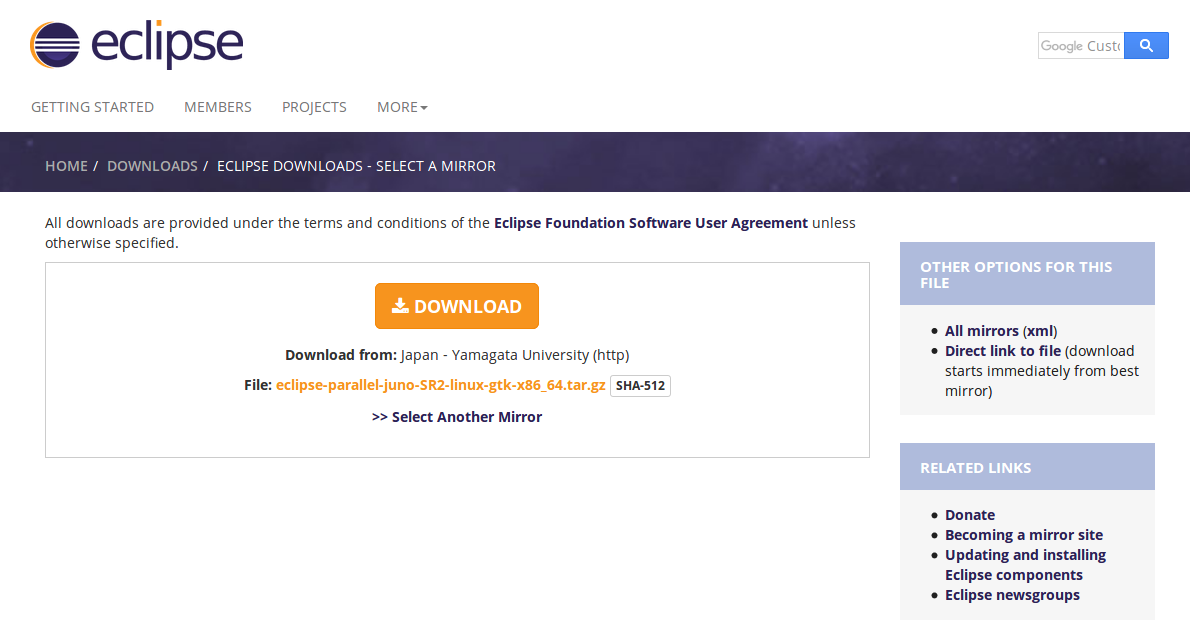
\includegraphics[width=0.8\textwidth]{Figure/AppendixA/eclipse-download-website.png}
	\rule{35em}{0.5pt}
	\caption[Eclipse Oxygen Download Official Website]{Eclipse Oxygen Download Official Website}
\end{figure}

Ensure the Eclipse IDE version selected is compatible with 64-bit Ubuntu Operating System.

\section{GoClipse plugin for Eclipse IDE installation}

\subsection{Eclipse Marketplace}

\begin{figure}[H]
	\centering
	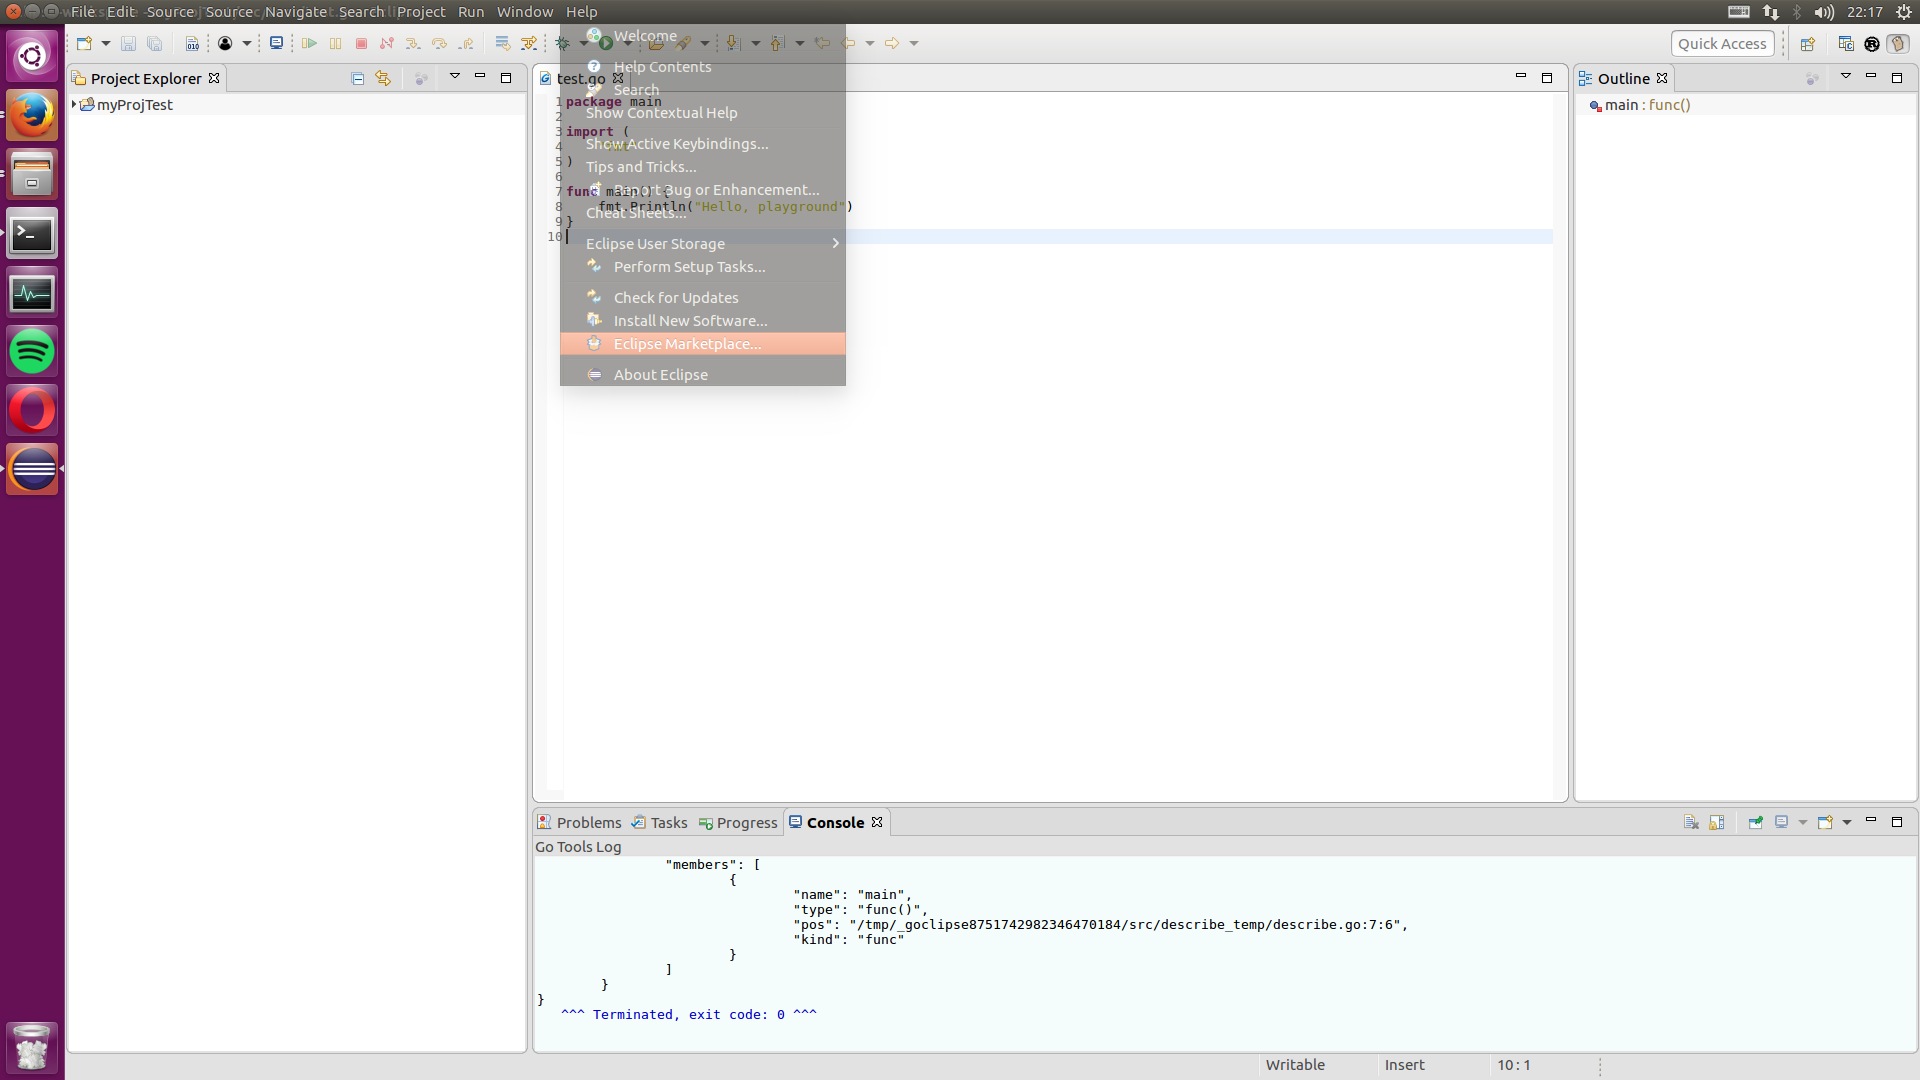
\includegraphics[width=0.8\textwidth]{Figure/AppendixA/goclipse-installation/goclipse-marketplace-1.png}
	\rule{35em}{0.5pt}
	\caption[Eclipse IDE Marketplace]{Eclipse IDE Marketplace}
\end{figure}

Open Eclipse Marketplace from Help and select Eclipse Marketplace to search for GoClipse plugin.

\subsection{Search Marketplace}

\begin{figure}[H]
	\centering
	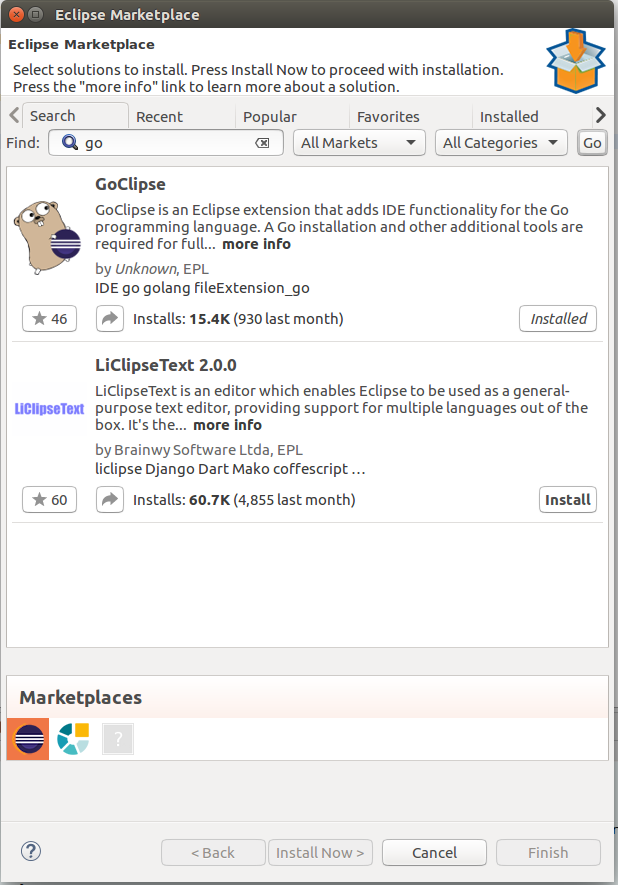
\includegraphics[width=0.3\textwidth]{Figure/AppendixA/goclipse-installation/goclipse-search-marketplace-2.png}
	\rule{35em}{0.5pt}
	\caption[Search Eclipse IDE Marketplace]{Search Eclipse IDE Marketplace}
\end{figure}

Type "Go" in search bar and press Go button to search for available plugin. Press install now to proceed with installation. 

\subsection{Open Perspective}

\begin{figure}[H]
	\centering
	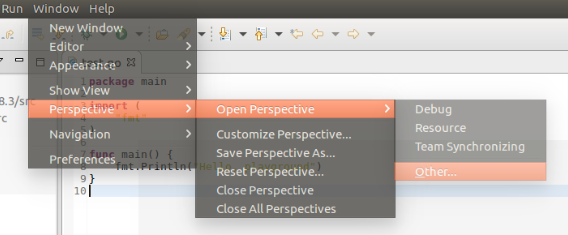
\includegraphics[width=0.5\textwidth]{Figure/AppendixA/goclipse-installation/goclipse-open-perspective-3.png}
	\rule{35em}{0.5pt}
	\caption[Open Perspective]{Open Perspective}
\end{figure}

After the installation is done and success, open Eclipse Perspective by select Window, Perspective, Open Perspective and choose Other.

\subsection{Choose Perspective}

\begin{figure}[H]
	\centering
	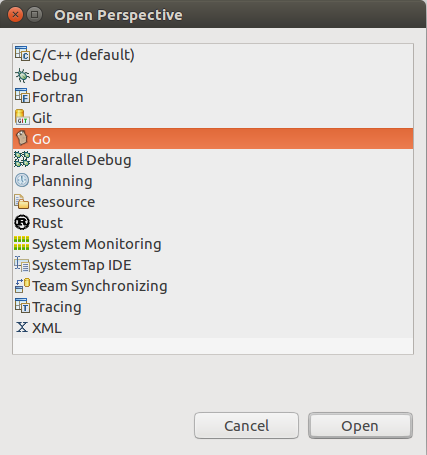
\includegraphics[width=0.8\textwidth]{Figure/AppendixA/goclipse-installation/goclipse-choose-4.png}
	\rule{35em}{0.5pt}
	\caption[Open Perspective]{Choose Go Perspective}
\end{figure}

Choose Go Perspective and press Enter. 

\subsection{Set Go compiler and GOPATH}

\begin{figure}[H]
	\centering
	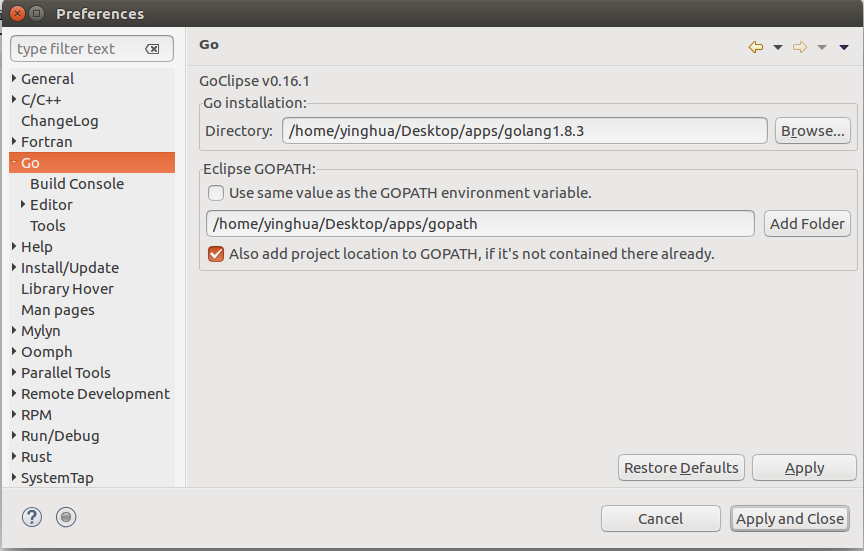
\includegraphics[width=0.8\textwidth]{Figure/AppendixA/goclipse-installation/5- goclipse-setting.png}
	\rule{35em}{0.5pt}
	\caption[Set Go compiler and GOPATH]{Set Go compiler and GOPATH}
\end{figure}

Set Go compiler  and GOPATH into Goclipse plugins. 

\subsection{Set GOCODE, GURU, GODEF and GOFMT path}

\begin{figure}[H]
	\centering
	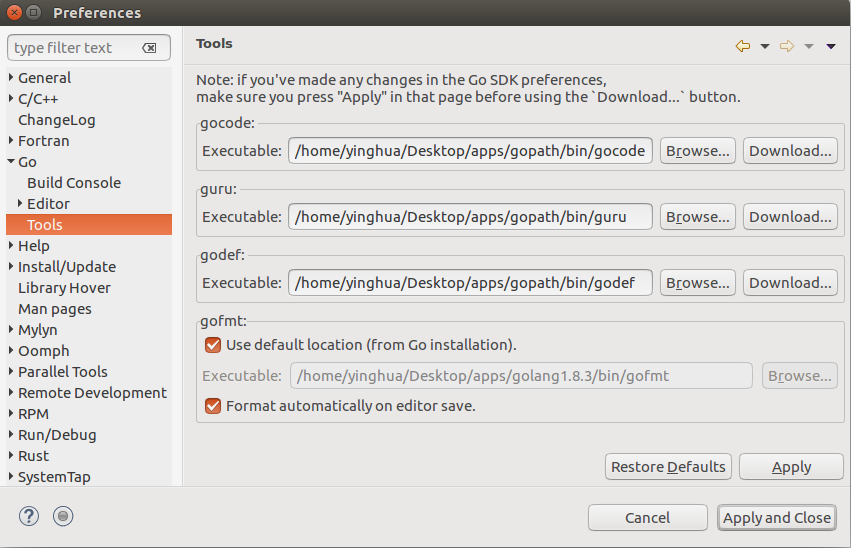
\includegraphics[width=0.8\textwidth]{Figure/AppendixA/goclipse-installation/6-goclipse-setting.png}
	\rule{35em}{0.5pt}
	\caption[Set GOCODE, GURU, GODEF and GOFMT path]{Set GOCODE, GURU, GODEF and GOFMT path}
\end{figure}

Set GOCODE, GURU, GODEF and GOFMT executable path into Goclipse plugins and press "Apply and Close" to complete the setup process. 

\subsection{Test Go compilation in Eclipse IDE}

\begin{figure}[H]
	\centering
	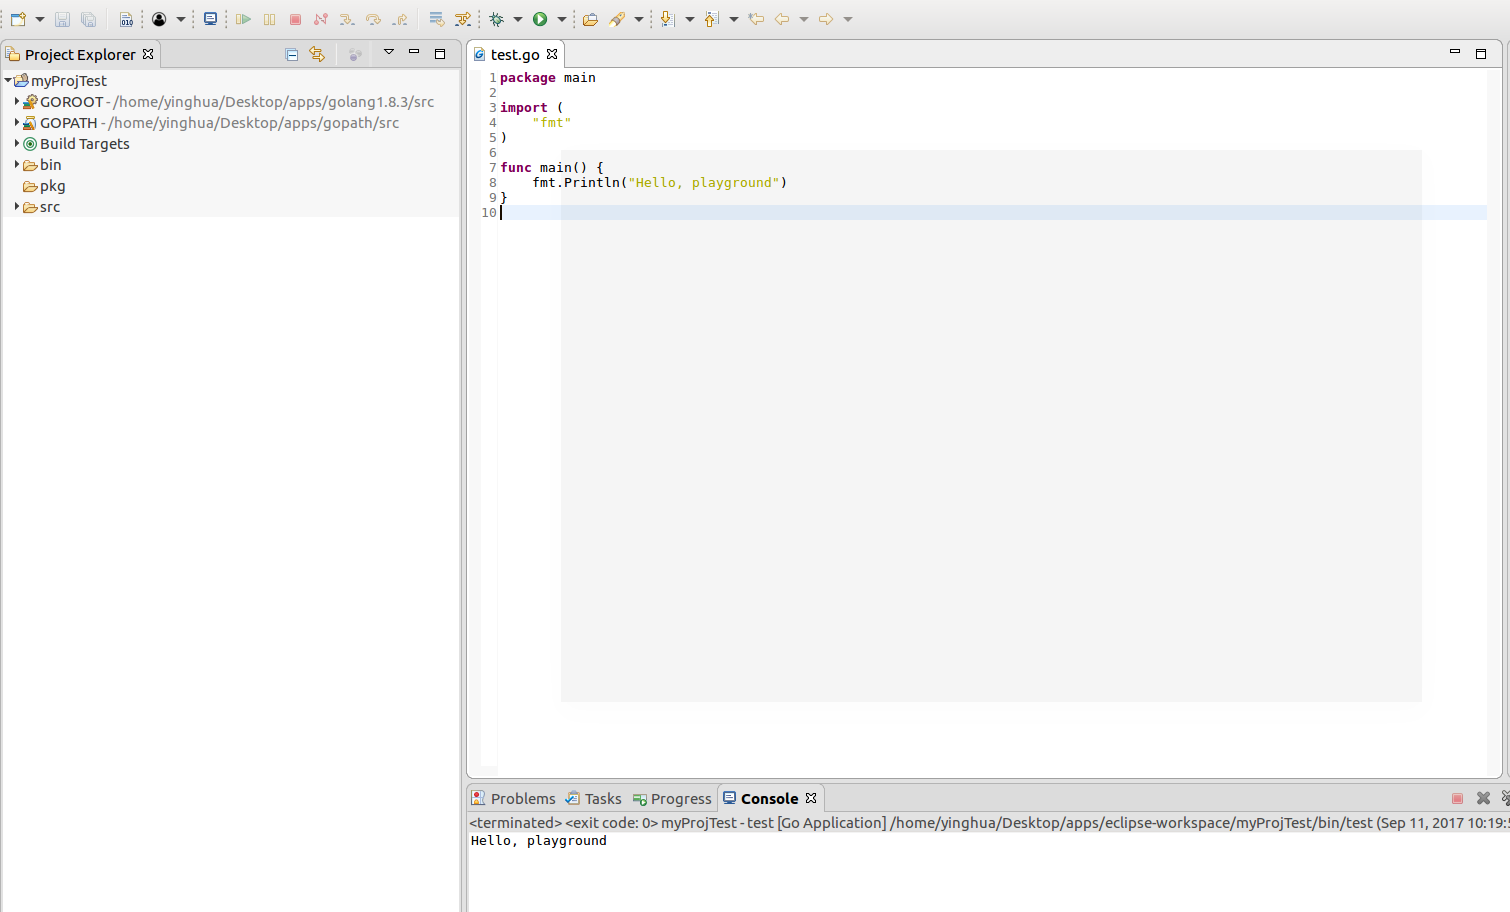
\includegraphics[width=0.8\textwidth]{Figure/AppendixA/goclipse-installation/7-goclipse-success.png}
	\rule{35em}{0.5pt}
	\caption[Test Go compilation in Eclipse IDE]{Test Go compilation in Eclipse IDE}
\end{figure}

Test Go compilation with simple Hello Playground program, the setup process is successful if the Go program is compile and run correctly. 

\section{RustDT plugin for Eclipse IDE installation}

\begin{figure}[H]
	\centering
	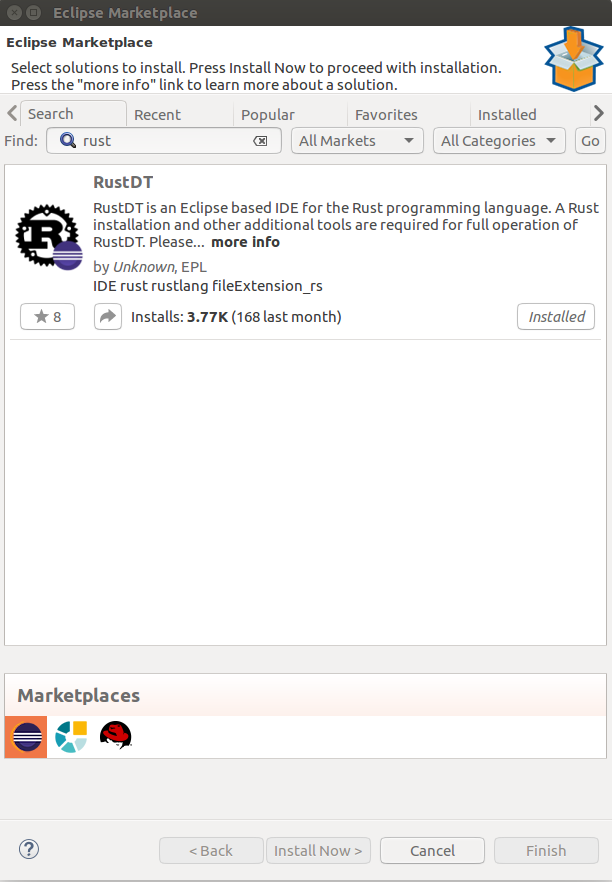
\includegraphics[width=0.6\textwidth]{Figure/AppendixA/rustdt-installation/1-rust-perspective.png}
	\rule{35em}{0.5pt}
	\caption[Test Go compilation in Eclipse IDE]{Test Go compilation in Eclipse IDE}
\end{figure}

Open Eclipse Marketplace similar to step in Appendix A.4.1 to A.4.7. Search the marketplace by type "Rust" in search bar and press Go button to search for tools. Press install now to proceed with installation. The setup process is similar with Goclipse installation process, once the installation and setup is done. The program will compile and run successfully.

\pagebreak  

\section{Linux command for PostgreSQL database installation}

\lstset{basicstyle=\ttfamily\tiny} 
\begin{lstlisting}[breaklines, frame=single, numbers=left, caption={Linux command for PostgreSQL database installation}, label=commandline-02]

===========================================
Step 1 - Install postgreSQL in command line 
===========================================

yinghua@yinghua-NL8C:~$ sudo apt-get update
yinghua@yinghua-NL8C:~$ sudo apt-get install postgresql postgresql-contrib
[sudo] password for yinghua: 

===========================================
Step 2 - Create database for FYP1 
===========================================
postgres=# create database fyp1;
CREATE DATABASE

postgres=# \l
List of databases
Name    |  Owner   | Encoding |   Collate   |    Ctype    |   Access privileges   
-----------+----------+----------+-------------+-------------+-----------------------
fyp1      | postgres | UTF8     | en_US.UTF-8 | en_US.UTF-8 | 
postgres  | postgres | UTF8     | en_US.UTF-8 | en_US.UTF-8 | 
template0 | postgres | UTF8     | en_US.UTF-8 | en_US.UTF-8 | =c/postgres          +
|          |          |             |             | postgres=CTc/postgres
template1 | postgres | UTF8     | en_US.UTF-8 | en_US.UTF-8 | =c/postgres          +
|          |          |             |             | postgres=CTc/postgres
(4 rows)

===========================================
Step 3 - Initial login with postgres user into psql
===========================================
yinghua@yinghua-NL8C:~$ sudo -i -u postgres psql 
psql (9.5.7)
Type "help" for help.

======================================================
Step 4 - Add myself as new user for PostgreSQL with Superuser access
======================================================
yinghua@yinghua-NL8C:~/Documents/FYP/Postcode-data/uk-postcodes-master$ sudo -i -u postgres psql fyp1
[sudo] password for yinghua: 
psql (9.5.7)
Type "help" for help.

postgres@yinghua-NL8C:~$ createuser -P -s -e yinghua
Enter password for new role: 
Enter it again: 
CREATE ROLE yinghua PASSWORD 'md5eec308d944ffa817c37ee6230b0c98eb' SUPERUSER CREATEDB CREATEROLE INHERIT LOGIN;

======================================================
Step 5 - List all the user in PostgreSQL
======================================================
postgres=# \du
List of roles
Role name |                         Attributes                         | Member of 
-----------+------------------------------------------------------------+-----------
postgres  | Superuser, Create role, Create DB, Replication, Bypass RLS | {}
yinghua   | Superuser, Create role, Create DB   


===========================================
Step 6 - Connect FYP1 Database
===========================================
postgres=# \c fyp1
You are now connected to database "fyp1" as user "postgres".

===============================================
Step 7 - Check whether there are tables in FYP1 database
===============================================
fyp1=# \dt
No relations found.

\end{lstlisting}

Install PostgreSQL database with command line using APT package. After the installation is success, create new user for new database in PostgreSQL. 


	
 








